\documentclass[12pt,english,dvipsnames,aspectratio=169,handout]{beamer}
\usepackage{fontspec}
\setsansfont[Mapping=tex-text]{Fira Sans}
\setcounter{secnumdepth}{4}
\setcounter{tocdepth}{4}
\usepackage[normalem]{ulem}
\usepackage[T1]{fontenc}
\usepackage{dcolumn}
\usepackage{booktabs}
\usepackage{setspace}
\makeatletter
\usetheme{metropolis}
\setbeamertemplate{frame footer}{Bosancianu | Schaub | Hertie School}
\setbeamerfont{page number in head/foot}{size=\tiny}
\setbeamercolor{footline}{fg=gray}
\usepackage{xcolor}
\usepackage{tikz}
\usetikzlibrary{arrows, positioning}
\usepackage[labelformat=empty]{caption}
% For table captions in Beamer
\usepackage[sectionbib]{apacite}
\renewcommand{\bibliographytypesize}{\footnotesize}
\makeatletter
\let\st@rtbibsection\@bibnewpage
\let\st@rtbibchapter\@bibnewpage
\makeatother
\usepackage{amsmath, mathtools}
\usepackage{xunicode}
\usepackage{hyperref}
\graphicspath{{./figures/}} 
% Defines a checkmark
\def\checkmark{\tikz\fill[scale=0.4,color=orange](0,.35) -- (.25,0) -- (1,.7) -- (.25,.15) -- cycle;}
% boxes
\def\boxitorange#1{%
	\smash{\color{orange}\fboxrule=1pt\relax\fboxsep=2pt\relax%
		\llap{\rlap{\fbox{\vphantom{0}\makebox[#1]{}}}~}}\ignorespaces
}
\def\boxitblue#1{%
	\smash{\color{blue}\fboxrule=1pt\relax\fboxsep=2pt\relax%
		\llap{\rlap{\fbox{\vphantom{0}\makebox[#1]{}}}~}}\ignorespaces
}
\newcommand{\indep}{\perp \!\!\!\! \perp}
\setbeamertemplate{itemize items}{\checkmark}
\usepackage{multirow}
\usepackage{subcaption}
\hypersetup{pdfauthor={Bosancianu and Schaub},
	pdftitle={Statistical Modeling and Causal Inference with R},
	pdfsubject={Week 4: Causal Graphs},
	pdfkeywords={Berlin, Hertie, 2020, week 4}}
\title{\textsc{Statistical Modeling and Causal Inference with R}}
\subtitle{Week 4: Causal Graphs}
\date{September 28, 2020}
\author{Manuel Bosancianu \hfill Max Schaub}
\institute{Hertie School}
\begin{document}
\maketitle

\begin{frame}
	\frametitle{Today's focus}
	
	\begin{itemize}
		\setlength\itemsep{1.5em}
		\item Causal graphs: components and terminology\bigskip
		\item Rules for independence: \textit{d-separation}\bigskip
		\item Examples!
	\end{itemize}
\end{frame}


\begin{frame}
	\frametitle{Last week}
	
	\begin{itemize}
		\item Linear regression as the most ``used and abused'' method in statistical inference
		\pause
		\item OLS (`ordinary least squares'') as the estimation method for $\beta$: the treatment effect (NATE)
		\pause
		\item Mechanics: finding the set of values which minimize the sum of squared residuals. 
	\end{itemize}

\begin{equation}
	Minimize: \sum_{i=1}^{n}(Y_i - \hat{\beta_0} - \underbrace{\hat{\beta_1}}_{NATE}X_i)^2
	\label{eq:01}
\end{equation}

\end{frame}


\begin{frame}
	\frametitle{Last week}
	
	\begin{equation}
		\footnotesize
		\underbrace{E[Y_{1i}|D_i = 1] - E[Y_{0i}|D_i = 0]}_{NATE} = \underbrace{\kappa}_{ATE} + \underbrace{E[u_i|D_i = 1] - E[u_i|D_i = 0]}_{Selection\; bias}
		\label{eq:02}
	\end{equation}

	Selection bias is a threat to recovering the ATE.
	
	\pause
	
	Regression can incorporate additional variables, in the quest for removing selection bias.
	
	\pause
	
	\textcolor{orange}{Limitations:} some confounders are difficult to measure, or are not present in the data.
	
\end{frame}


\section{Causal graphs}

\begin{frame}
	\frametitle{Why bother with graphs?}
	\textit{Controlling} for confounders can eliminate \textit{selection bias}, \textcolor{orange}{but} how do we \underline{choose} the confounders?\bigskip
	
	Should we control for everything we can measure?\bigskip
	
	\pause
	
	Causal graphs:
	\begin{itemize}
		\item provide an concise account of the DGP
		\item allow us to decide which controls to include
		\item offer a framework to discuss all aspects of causal inference (experimental and observational)
	\end{itemize}
	
\end{frame}


\begin{frame}
	\frametitle{Building blocks}
	Variables are the \textcolor{orange}{nodes} (or \textit{vertices}) of the graph.
	
	\begin{figure}
		\centering
		\scriptsize
		\begin{tikzpicture}[->,
			>=stealth',
			shorten >=1pt,
			auto,
			thick]
			
			\draw[fill=black, draw=black] (0,0) circle (0.8ex) node (a) [below, yshift=-0.2cm] {\large\texttt{X}};
			\draw[fill=black, draw=black] (2,0) circle (0.8ex) node (a) [below, yshift=-0.2cm] {\large\texttt{Y}};
		\end{tikzpicture}
	\end{figure}\bigskip

	\pause
	
	Links between nodes are called \textcolor{orange}{edges} (or \textit{arcs}).
	
	\begin{figure}
		\centering
		\scriptsize
		\begin{tikzpicture}[->,
			>=stealth',
			shorten >=1pt,
			auto,
			thick]
			
			\draw[fill=black, draw=black] (0,0) circle (0.8ex) node (a) [below, yshift=-0.2cm] {\large\texttt{X}};
			\draw[fill=black, draw=black] (2,0) circle (0.8ex) node (b) [below, yshift=-0.2cm] {\large\texttt{Y}};
			\draw[->, black] (0,0) -- (1.92,0);
		\end{tikzpicture}
	\end{figure}
	
\end{frame}


\begin{frame}
	\frametitle{Implications}
	
	\begin{figure}
		\centering
		\scriptsize
		\begin{tikzpicture}[->,
			>=stealth',
			shorten >=1pt,
			auto,
			thick]
			
			\draw[fill=black, draw=black] (0,0) circle (0.8ex) node (a) [below, yshift=-0.2cm] {\large\texttt{X}};
			\draw[fill=black, draw=black] (2,0) circle (0.8ex) node (b) [below, yshift=-0.2cm] {\large\texttt{Y}};
			\draw[->, black] (0,0) -- (1.92,0);
		\end{tikzpicture}
	\end{figure}
	
	\begin{itemize}
		\item time flows from left to right
		
		\pause
		
		\item presence of an edge means a direct causal effect from \texttt{X} to \texttt{Y}
		
		\pause
		
		\item absence of an edge suggests the \textit{lack} of a direct causal effect
	\end{itemize}\bigskip
	
	\pause
	
	Directed edge means \texttt{X} is \textcolor{orange}{parent} and \texttt{Y} is \textcolor{orange}{child}.
	
\end{frame}


\begin{frame}
	\frametitle{More complexity}
	
	\begin{figure}
		\centering
		\scriptsize
		\begin{tikzpicture}[->,
			>=stealth',
			shorten >=1pt,
			auto,
			thick]
			
			\draw[fill=black, draw=black] (0,0) circle (0.8ex) node (a) [below, yshift=-0.2cm] {\large\texttt{X}};
			\draw[fill=black, draw=black] (2,0) circle (0.8ex) node (b) [below, yshift=-0.2cm] {\large\texttt{Y}};
			\draw[fill=black, draw=black] (1,1.5) circle (0.8ex) node (b) [above, yshift=0.2cm] {\large\texttt{C}};
			\draw[->, black] (0,0) -- (1.92,0);
			\draw[->, black] (1,1.5) -- (0,0.08);
			\draw[->, black] (1,1.5) -- (1.94,0.06);
		\end{tikzpicture}
	\end{figure} \bigskip

	\pause

	Nodes that are only parents are called \textcolor{orange}{exogenous} (or \textit{root} nodes).\bigskip
	
	Nodes that are both parent and child are called \textcolor{orange}{endogenous}.
	
\end{frame}


\begin{frame}
	\frametitle{DAGs}
	
	\begin{figure}
		\centering
		\scriptsize
		\begin{tikzpicture}[->,
			>=stealth',
			shorten >=1pt,
			auto,
			thick]
			
			\draw[fill=black, draw=black] (0,0) circle (0.8ex) node (a) [below, yshift=-0.2cm] {\large\texttt{X}};
			\draw[fill=black, draw=black] (2,0) circle (0.8ex) node (b) [below, yshift=-0.2cm] {\large\texttt{Y}};
			\draw[fill=black, draw=black] (1,1.5) circle (0.8ex) node (b) [above, yshift=0.2cm] {\large\texttt{C}};
			\draw[->, black] (0,0) -- (1.92,0);
			\draw[->, black] (1,1.5) -- (0,0.08);
			\draw[->, black] (1,1.5) -- (1.94,0.06);
		\end{tikzpicture}
	\end{figure}
	
	We focus on a special type of causal model: the \textcolor{orange}{directed acyclic graph}.

	\pause
	
	\begin{itemize}
		\item \underline{directed}: the edges all have directions
		\item \underline{acyclic}: variable cannot cause itself, through another variable (or variables)
	\end{itemize}
	
\end{frame}


\begin{frame}
	\frametitle{Typology of nodes}
	A few foundational configurations in a DAG.
	
	\begin{figure}
		\centering
		\scriptsize
		\begin{tikzpicture}[->,
			>=stealth',
			shorten >=1pt,
			auto,
			thick]
			
			\draw[fill=black, draw=black] (0,0) circle (0.8ex) node (a) [below, yshift=-0.2cm] {\large\texttt{X}};
			\draw[fill=black, draw=black] (2,0) circle (0.8ex) node (b) [below, yshift=-0.2cm] {\large\texttt{Y}};
			\draw[fill=black, draw=black] (1,1.5) circle (0.8ex) node (b) [above, yshift=0.2cm] {\large\texttt{C}};
			\draw[->, black] (0,0) -- (1.92,0);
			\draw[->, black] (1,1.5) -- (0,0.08);
			\draw[->, black] (1,1.5) -- (1.94,0.06);
		\end{tikzpicture}
	\end{figure}\bigskip

	\pause

	\texttt{C} is a \textcolor{orange}{confounder}: causal impact on both treatment assignment and outcome.
	
\end{frame}



\begin{frame}
	\frametitle{Typology of nodes}

	\begin{figure}
		\centering
		\scriptsize
		\begin{subfigure}{0.45\linewidth}
		\begin{tikzpicture}[->,
			>=stealth',
			shorten >=1pt,
			auto,
			thick]
			
			\draw[fill=black, draw=black] (0,0) circle (0.8ex) node (a) [below, yshift=-0.2cm] {\large\texttt{X}};
			\draw[fill=black, draw=black] (2,0) circle (0.8ex) node (b) [below, yshift=-0.2cm] {\large\texttt{Y}};
			\draw[fill=black, draw=black] (1,1.5) circle (0.8ex) node (b) [above, yshift=0.2cm] {\large\texttt{C}};
			\draw[->, black] (0,0) -- (1.92,0);
			\draw[->, black] (0,0) -- (0.95,1.45);
			\draw[->, black] (1,1.5) -- (1.94,0.06);
		\end{tikzpicture}
		\end{subfigure}
		\begin{subfigure}{0.45\linewidth}
		\begin{tikzpicture}[->,
			>=stealth',
			shorten >=1pt,
			auto,
			thick]
			
			\draw[fill=black, draw=black] (0,0.75) circle (0.8ex) node (a) [below, yshift=-0.2cm] {\large\texttt{X}};
			\draw[fill=black, draw=black] (2,0.75) circle (0.8ex) node (b) [below, yshift=-0.2cm] {\large\texttt{C}};
			\draw[fill=black, draw=black] (4,0.75) circle (0.8ex) node (b) [below, yshift=-0.2cm] {\large\texttt{Y}};
			\draw[->, black] (0,0.75) -- (1.92,0.75);
			\draw[->, black] (2,0.75) -- (3.92,0.75);
		\end{tikzpicture}
		\end{subfigure}
	\end{figure}\bigskip
	
	\texttt{C} is a \textcolor{orange}{mediator}: carries part or all of the effect of \texttt{X} on \texttt{Y}.
	
\end{frame}


\begin{frame}
	\frametitle{Typology of nodes}

	\begin{figure}
		\centering
		\scriptsize
		\begin{tikzpicture}[->,
			>=stealth',
			shorten >=1pt,
			auto,
			thick]
			
			\draw[fill=black, draw=black] (0,0) circle (0.8ex) node (a) [below, yshift=-0.2cm] {\large\texttt{X}};
			\draw[fill=black, draw=black] (2,0) circle (0.8ex) node (b) [below, yshift=-0.2cm] {\large\texttt{Y}};
			\draw[fill=black, draw=black] (1,1.5) circle (0.8ex) node (b) [above, yshift=0.2cm] {\large\texttt{C}};
			\draw[->, black] (0,0) -- (1.92,0);
			\draw[->, black] (0,0) -- (0.95,1.42);
			\draw[->, black] (2,0) -- (1.05,1.42);
		\end{tikzpicture}
	\end{figure}\bigskip
	
	\texttt{C} is a \textcolor{orange}{collider}: a common child node of at least two parent nodes.
	
\end{frame}


\begin{frame}
	\frametitle{Paths}
	
	\begin{figure}
		\scriptsize
		\begin{subfigure}{0.32\linewidth}
			\centering
			\begin{tikzpicture}[->,
				>=stealth',
				shorten >=1pt,
				auto,
				thick]
				
				\draw[fill=black, draw=black] (0,0) circle (0.8ex) node (a) [below, yshift=-0.2cm] {\large\texttt{X}};
				\draw[fill=black, draw=black] (2,0) circle (0.8ex) node (b) [below, yshift=-0.2cm] {\large\texttt{Y}};
				\draw[fill=black, draw=black] (1,1.5) circle (0.8ex) node (b) [above, yshift=0.2cm] {\large\texttt{C}};
				\draw[->, orange] (0.12,0) -- (1.92,0);
				\draw[->, black] (0,0) -- (0.95,1.45);
				\draw[->, black] (1,1.5) -- (1.94,0.06);
			\end{tikzpicture}
			\subcaption{Direct path}
		\end{subfigure}
		\begin{subfigure}{0.32\linewidth}
			\centering
			\begin{tikzpicture}[->,
				>=stealth',
				shorten >=1pt,
				auto,
				thick]
				
				\draw[fill=black, draw=black] (0,0) circle (0.8ex) node (a) [below, yshift=-0.2cm] {\large\texttt{X}};
				\draw[fill=black, draw=black] (2,0) circle (0.8ex) node (b) [below, yshift=-0.2cm] {\large\texttt{Y}};
				\draw[fill=black, draw=black] (1,1.5) circle (0.8ex) node (b) [above, yshift=0.2cm] {\large\texttt{C}};
				\draw[->, black] (0,0) -- (1.92,0);
				\draw[->, orange] (0,0.12) -- (0.95,1.45);
				\draw[->, orange] (1.05,1.38) -- (1.94,0.06);
			\end{tikzpicture}
			\subcaption{Front-door path}
			\end{subfigure}
			\begin{subfigure}{0.32\linewidth}
				\centering
				\begin{tikzpicture}[->,
					>=stealth',
					shorten >=1pt,
					auto,
					thick]
					
					\draw[fill=black, draw=black] (0,0) circle (0.8ex) node (a) [below, yshift=-0.2cm] {\large\texttt{X}};
					\draw[fill=black, draw=black] (2,0) circle (0.8ex) node (b) [below, yshift=-0.2cm] {\large\texttt{Y}};
					\draw[fill=black, draw=black] (1,1.5) circle (0.8ex) node (b) [above, yshift=0.2cm] {\large\texttt{C}};
					\draw[->, black] (0,0) -- (1.92,0);
					\draw[->, orange] (0.95,1.42) -- (0.05,0.05);
					\draw[->, orange] (1.05,1.42) -- (1.95,0.05);
				\end{tikzpicture}
				\subcaption{Back-door path}
		\end{subfigure}
	\end{figure}

	\pause
	
	Whether a causal path is \textcolor{orange}{open} or \textcolor{orange}{closed} depends on:
	\begin{enumerate}
		\item whether or not we control for nodes on the path in our analysis
		\item what type of nodes we control for (colliders, confounders, or mediators)
	\end{enumerate}
	
\end{frame}


\begin{frame}
	\frametitle{Paths}
	\begin{figure}
		\begin{tikzpicture}[->,
			>=stealth',
			shorten >=1pt,
			auto,
			thick]
			
			\draw[fill=black, draw=black] (0,0.75) circle (0.6ex) node (a) [below, yshift=-0.2cm] {\large\texttt{A}};
			\draw[fill=black, draw=black] (2,0.75) circle (0.6ex) node (b) [below, yshift=-0.2cm] {\large\texttt{B}};
			\draw[fill=black, draw=black] (4,0.75) circle (0.6ex) node (b) [below, yshift=-0.2cm] {\large\texttt{C}};
			\draw[fill=black, draw=black] (6,0.75) circle (0.6ex) node (b) [below, yshift=-0.2cm] {\large\texttt{D}};
			\draw[->, black] (0,0.75) -- (1.92,0.75);
			\draw[->, black] (2,0.75) -- (3.92,0.75);
			\draw[->, black] (4,0.75) -- (5.92,0.75);
		\end{tikzpicture}
	\end{figure}
	
	With longer paths, we have \textcolor{orange}{ancestors} and \textcolor{orange}{descendants}.\bigskip
	
	\texttt{A} is an ancestor for \texttt{B}, \texttt{C}, and \texttt{D}. The latter are all descendants for \texttt{A}.\bigskip
	
	\pause
	
	The path from \texttt{A} to \texttt{D} is \textcolor{orange}{causal}. The path from \texttt{P} to \texttt{S} is \textcolor{orange}{non-causal}.
	
	\begin{figure}
		\begin{tikzpicture}[->,
			>=stealth',
			shorten >=1pt,
			auto,
			thick]
			
			\draw[fill=black, draw=black] (0,0.75) circle (0.6ex) node (a) [below, yshift=-0.2cm] {\large\texttt{P}};
			\draw[fill=black, draw=black] (2,0.75) circle (0.6ex) node (b) [below, yshift=-0.2cm] {\large\texttt{Q}};
			\draw[fill=black, draw=black] (4,0.75) circle (0.6ex) node (b) [below, yshift=-0.2cm] {\large\texttt{R}};
			\draw[fill=black, draw=black] (6,0.75) circle (0.6ex) node (b) [below, yshift=-0.2cm] {\large\texttt{S}};
			\draw[->, black] (0,0.75) -- (1.92,0.75);
			\draw[->, black] (2,0.75) -- (3.92,0.75);
			\draw[->, orange] (5.88,0.75) -- (4.08,0.75);
		\end{tikzpicture}
	\end{figure}
	
\end{frame}


\section{Example \#1}

\begin{frame}
	\frametitle{Relative power theory}
	Proposed by \citeA{goodin_rational_1980} as an explanation for why poorer people participate less in politics.
	
	\begin{figure}
		\begin{spacing}{0.5}
		\begin{tikzpicture}[->,
			>=stealth',
			shorten >=1pt,
			auto,
			thick]
			\node at (0,6) (a) [text width = 1.75cm] {\scriptsize Government dependency};
			\node at (0,5) (b) [text width = 1.75cm] {\scriptsize Government responsibility};
	     	\node at (3,5.5) (c) [text width = 1.75cm] {\scriptsize Utility of participation};
			\node at (5,4) (d) [text width = 1.75cm] {\scriptsize Information};
			\node at (9,4) (e) [text width = 1.75cm] {\scriptsize Participation};
			\node at (3,2.5) (f) [text width = 1.75cm] {\scriptsize Relative power};
			\node at (0,2) (g) [text width = 1.75cm] {\scriptsize Income position};
			\draw[->, black] (a) -- (c);
			\draw[->, black] (b) -- (c);
			\draw[->, black] (c) -- (d);
			\draw[->, black] (c) -- (e);
			\draw[->, black] (d) -- (e);
			\draw[->, black] (g) -- (f);
			\draw[->, black] (f) -- (d);
			\draw[->, black] (f) -- (e);
		\end{tikzpicture}
	    \end{spacing}
	\end{figure}
	
\end{frame}

\begin{frame}
	\frametitle{Stylized}
		\begin{minipage}[t]{0.50\linewidth}
			\begin{figure}
				\centering
				\begin{tikzpicture}[->,
					>=stealth',
					shorten >=1pt,
					auto,
					thick]
					\node at (0,6) (a) {GD};
					\node at (0,5) (b) {GR};
					\node at (2,5.5) (c) {UP};
					\node at (3,4) (d) {I};
					\node at (4.5,4) (e) {P};
					\node at (2,2.5) (f) {RP};
					\node at (0,2) (g) {IP};
					\draw[->, black] (a) -- (c);
					\draw[->, black] (b) -- (c);
					\draw[->, black] (c) -- (d);
					\draw[->, black] (c) -- (e);
					\draw[->, black] (d) -- (e);
					\draw[->, black] (g) -- (f);
					\draw[->, black] (f) -- (d);
					\draw[->, black] (f) -- (e);
				\end{tikzpicture}
			\end{figure}
	\end{minipage}
		\begin{minipage}[t]{0.48\linewidth}
			How many paths from RP to P?
			
			\pause
			
			\begin{itemize}
				\item RP $\rightarrow$ P
				\item RP $\rightarrow$ I $\rightarrow$ P 
				\item RP $\rightarrow$ I $\leftarrow$ UP $\rightarrow$ P 
			\end{itemize}
		
			\pause
			
			How many causal/ non-causal?
			
			\begin{itemize}
				\item 1 \& 2 causal
				\item 3 non-causal 
			\end{itemize}
		
		\end{minipage}
	
\end{frame}



\begin{frame}
	\frametitle{Stylized}
	\begin{minipage}[t]{0.50\linewidth}
		\begin{figure}
			\centering
			\begin{tikzpicture}[->,
				>=stealth',
				shorten >=1pt,
				auto,
				thick]
				\node at (0,6) (a) {GD};
				\node at (0,5) (b) {GR};
				\node at (2,5.5) (c) {UP};
				\node at (3,4) (d) {I};
				\node at (4.5,4) (e) {P};
				\node at (2,2.5) (f) {RP};
				\node at (0,2) (g) {IP};
				\draw[->, black] (a) -- (c);
				\draw[->, black] (b) -- (c);
				\draw[->, black] (c) -- (d);
				\draw[->, black] (c) -- (e);
				\draw[->, black] (d) -- (e);
				\draw[->, black] (g) -- (f);
				\draw[->, black] (f) -- (d);
				\draw[->, black] (f) -- (e);
			\end{tikzpicture}
		\end{figure}
	\end{minipage}
	\begin{minipage}[t]{0.48\linewidth}
		How many exogenous nodes?
		
		\pause
		
		3: \texttt{GD}, \texttt{GR}, \texttt{IP}
		\bigskip
		\pause
		
		How many endogenous?
		
		\pause
		
		4: \texttt{UP}, \texttt{RP}, \texttt{I}, \texttt{P} 
		\bigskip
		\pause
		
		How many back-door paths (from \texttt{RP} to \texttt{P})?
		
		\pause
		
		In this case, none.
		
	\end{minipage}
	
\end{frame}


\begin{frame}
	\frametitle{Stylized}
	\begin{minipage}[t]{0.50\linewidth}
		\begin{figure}
			\centering
			\begin{tikzpicture}[->,
				>=stealth',
				shorten >=1pt,
				auto,
				thick]
				\node at (0,6) (a) {GD};
				\node at (0,5) (b) {GR};
				\node at (2,5.5) (c) {UP};
				\node at (3,4) (d) {I};
				\node at (4.5,4) (e) {P};
				\node at (2,2.5) (f) {RP};
				\node at (0,2) (g) {IP};
				\draw[->, black] (a) -- (c);
				\draw[->, black] (b) -- (c);
				\draw[->, black] (c) -- (d);
				\draw[->, black] (c) -- (e);
				\draw[->, black] (d) -- (e);
				\draw[->, black] (g) -- (f);
				\draw[->, black] (f) -- (d);
				\draw[->, black] (f) -- (e);
			\end{tikzpicture}
		\end{figure}
	\end{minipage}
	\begin{minipage}[t]{0.48\linewidth}
		How many colliders?
		
		\pause
		
		2: \texttt{I}, \texttt{UP}
		\bigskip
		\pause
		
		How many confounders (if we want the effect of \texttt{I} on \texttt{P})?
		
		\pause
		
		2: \texttt{UP}, \texttt{RP}
		\bigskip
		\pause
		
		How many mediators (if we want the effect of \texttt{IP} on \texttt{P})?
		
		\pause
		
		2: \texttt{RP}, \texttt{I}
		
	\end{minipage}
	
\end{frame}


\section{d-separation}


\begin{frame}
	\frametitle{Linkage to regression}
	$\beta$ is unbiased if $E[u_i |D_i] = 0$ (``0 conditional mean assumption'').
	
	\pause
	
	Reformulating: treatment assignment should be unaffected by selection bias.
	
	\begin{figure}
		\centering
		\begin{tikzpicture}[->,
			>=stealth',
			shorten >=1pt,
			auto,
			thick]
			
			\draw[fill=black, draw=black] (0,0) circle (0.6ex) node (a) [below, yshift=-0.2cm] {\large\texttt{D}};
			\draw[fill=black, draw=black] (2,0) circle (0.6ex) node (b) [below, yshift=-0.2cm] {\large\texttt{Y}};
			\draw[fill=black, draw=black] (1,1.5) circle (0.6ex) node (b) [above, yshift=0.2cm] {\large\texttt{C}};
			\draw[->, orange] (0.12,0) -- (1.92,0);
			\draw[->, black] (1,1.5) -- (0.05,0.1)  node [midway,xshift=-0.3cm,yshift=0.27cm] {\textcolor{orange}{$\times$}};
			\draw[->, black] (1.05,1.38) -- (1.94,0.06) node [midway,xshift=-0.3cm,yshift=-0.27cm] {\textcolor{orange}{$\times$}};
		\end{tikzpicture}
	\end{figure}

	\pause
	
	Treatment assignment should be as good as random.
	
\end{frame}


\begin{frame}
	\frametitle{Closing open back-door paths}
	\begin{figure}
		\centering
		\begin{tikzpicture}[->,
			>=stealth',
			shorten >=1pt,
			auto,
			thick]
			
			\draw[fill=black, draw=black] (0,0) circle (0.6ex) node (a) [below, yshift=-0.2cm] {\large\texttt{D}};
			\draw[fill=black, draw=black] (2,0) circle (0.6ex) node (b) [below, yshift=-0.2cm] {\large\texttt{Y}};
			\draw[fill=black, draw=black] (1,1.5) circle (0.6ex) node (b) [above, yshift=0.2cm] {\large\texttt{C}};
			\draw[->, orange] (0.12,0) -- (1.92,0);
			\draw[->, black] (1,1.5) -- (0.05,0.1);
			\draw[->, black] (1.05,1.38) -- (1.94,0.06);
		\end{tikzpicture}
	\end{figure}
	
	$D \rightarrow Y$ is what we're trying to capture.\bigskip
	
	\pause
	
	$D \leftarrow C \rightarrow Y$ is a spurious source of association between \texttt{D} and \texttt{Y}.
	
\end{frame}


\begin{frame}
	\frametitle{Back-door criterion}
	To compute $NATE = E[Y_{1i} | D_i=1] - E[Y_{0i} | D_i=0]$, we need to isolate the direct path: $D \rightarrow Y$.\bigskip
	
	\pause
	
	Open backdoor paths create spurious correlations between \texttt{D} and \texttt{Y}.\bigskip
	
	\pause
	
	2 strategies to close them:
	
	\begin{itemize}
		\item If path contains confounder, \textcolor{orange}{condition} on confounder
		\item if path contains collider it is already closed, so \textcolor{orange}{do not condition} on collider
	\end{itemize}
	
\end{frame}


\begin{frame}
	\frametitle{Canonical configurations: confounders}
	\begin{figure}
		\centering
		\begin{tikzpicture}[->,
			>=stealth',
			shorten >=1pt,
			auto,
			thick]
			
			\draw[fill=black, draw=black] (0,0) circle (0.6ex) node (a) [below, yshift=-0.2cm] {\large\texttt{D}};
			\draw[fill=black, draw=black] (2,0) circle (0.6ex) node (b) [below, yshift=-0.2cm] {\large\texttt{Y}};
			\draw[fill=black, draw=black] (1,1.5) circle (0.6ex) node (b) [above, yshift=0.2cm] {\large\texttt{C}};
			\draw[->, orange] (0.12,0) -- (1.92,0);
			\draw[->, black] (1,1.5) -- (0.05,0.1);
			\draw[->, black] (1.05,1.38) -- (1.94,0.06);
		\end{tikzpicture}
	\end{figure}
	
	$D \leftarrow C \rightarrow Y$ is an \textcolor{orange}{open} back-door path (\texttt{C} is not a collider).\bigskip
	
	\pause
	
	\textcolor{orange}{Solution}: condition on \texttt{C} to close the path.
	
	\begin{equation}
		Y_i = \beta_0 + \beta_1D_i + \beta_2C_i + \epsilon_i
	\end{equation}
	
\end{frame}


\begin{frame}
	\frametitle{Canonical configurations: mediators}
	\begin{figure}
		\centering
		\begin{tikzpicture}[->,
			>=stealth',
			shorten >=1pt,
			auto,
			thick]
			
			\draw[fill=black, draw=black] (0,0.75) circle (0.8ex) node (a) [below, yshift=-0.2cm] {\large\texttt{D}};
			\draw[fill=black, draw=black] (2,0.75) circle (0.8ex) node (b) [below, yshift=-0.2cm] {\large\texttt{C}};
			\draw[fill=black, draw=black] (4,0.75) circle (0.8ex) node (b) [below, yshift=-0.2cm] {\large\texttt{Y}};
			\draw[->, black] (0,0.75) -- (1.92,0.75);
			\draw[->, black] (2,0.75) -- (3.92,0.75);
		\end{tikzpicture}
	\end{figure}

	\pause
	
	$D \rightarrow C \rightarrow Y$: causal path between treatment and outcome.\bigskip
	
	\pause
	
	\textcolor{orange}{Solution}: do not condition on C, to keep the path open.\bigskip
	
	\pause
	
	Rules:
	
	\begin{itemize}
		\item close all non-causal paths linking \texttt{D} to \texttt{Y}
		\item do not close any causal path between \texttt{D} and \texttt{Y}
	\end{itemize}
	
	
\end{frame}




\begin{frame}
	\frametitle{Canonical configurations: colliders}
	\begin{figure}
		\centering
	\begin{tikzpicture}[->,
		>=stealth',
		shorten >=1pt,
		auto,
		thick]
		
		\draw[fill=black, draw=black] (0,0) circle (0.8ex) node (a) [below, yshift=-0.2cm] {\large\texttt{D}};
		\draw[fill=black, draw=black] (2,0) circle (0.8ex) node (b) [below, yshift=-0.2cm] {\large\texttt{Y}};
		\draw[fill=black, draw=black] (1,1.5) circle (0.8ex) node (b) [above, yshift=0.2cm] {\large\texttt{C}};
		\draw[->, orange] (0.15,0) -- (1.92,0);
		\draw[->, black] (0.05,0.12) -- (0.95,1.45);
		\draw[->, black] (1.95,0.12) -- (1.05,1.45);
	\end{tikzpicture}
	\end{figure}
	
	\pause
	
	$D \rightarrow C \leftarrow Y$: noncausal path between treatment and outcome.\bigskip
	
	\pause
	
	\textcolor{orange}{Solution}: do not condition on C, as path is closed already.\bigskip
	
	\pause
	
	Don't condition on a descendant of a collider, either \cite[p.~44-45]{pearl_causal_2016}.
	
\end{frame}



\begin{frame}
	\frametitle{Strategy for \textit{d}-separation}
	A few simple steps \cite[p.~73]{cunningham_causal_2021}:
	
	\begin{enumerate}
		\item write down all paths between \texttt{D} and \texttt{Y}
		
		\pause
		
		\item identify open/closed back-door paths (any confounders or colliders?)
		
		\pause
		
		\item find conditioning strategy that closes all open back-doors
	\end{enumerate}
	
	\pause
	
	Last step is not always possible.

	\pause

	When all non-causal paths between \texttt{D} and \texttt{Y} are blocked, \texttt{D} and \texttt{Y} are \textcolor{orange}{d-separated}.
		
\end{frame}



\section{Example \#2}

\begin{frame}
	\frametitle{Google gender pay discrimination}
	
	\begin{figure}
		\centering
		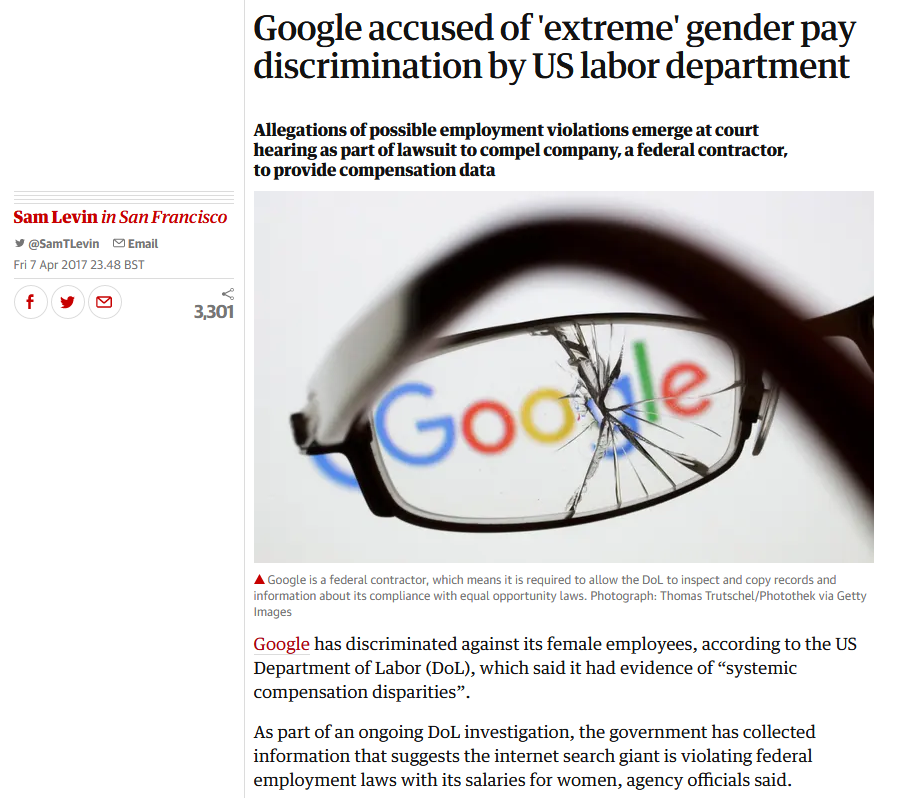
\includegraphics[scale=0.3]{../04-figures/04/04-01}
	\end{figure}
	
\end{frame}


\begin{frame}
	\frametitle{Google gender pay discrimination}
	
	\begin{figure}
		\centering
		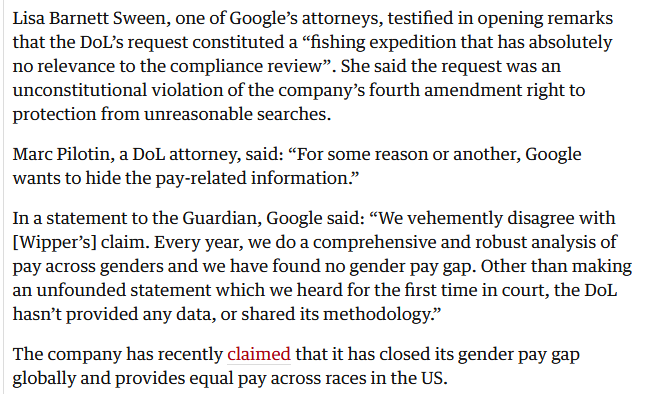
\includegraphics[scale=0.4]{../04-figures/04/04-02}
	\end{figure}
	As a federal contractor Google has to share data relevant to equal opportunity law compliance, if asked.\bigskip
	
	The company initially resisted the DoL request.
\end{frame}

\begin{frame}
	\frametitle{Google performs internal analysis}
	
	\begin{figure}
		\centering
		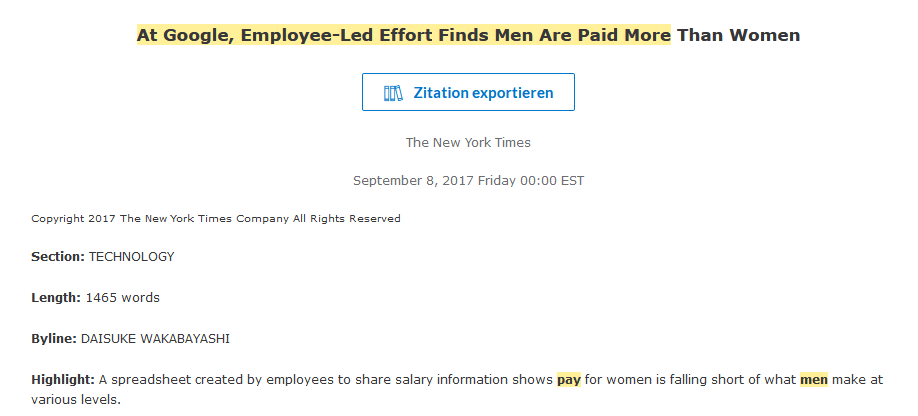
\includegraphics[scale=0.3]{../04-figures/04/04-03}
    	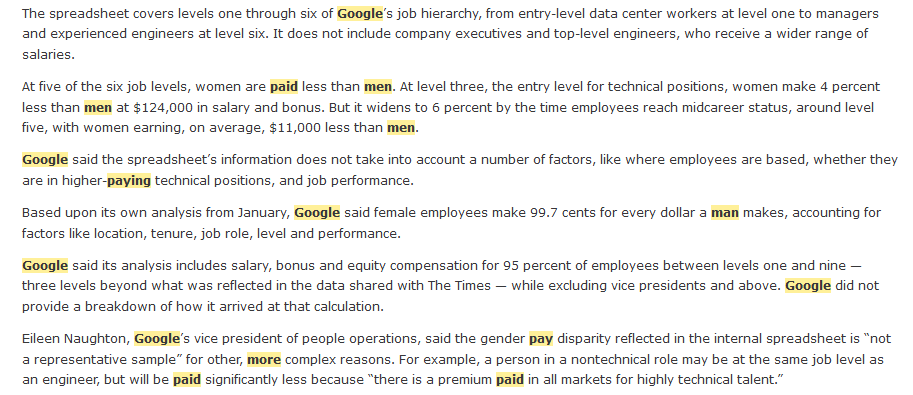
\includegraphics[scale=0.3]{../04-figures/04/04-04}
	\end{figure}
\end{frame}


\begin{frame}
	\frametitle{Who is right?}
	\begin{figure}
		\centering
		\scriptsize
		\begin{tikzpicture}[->,
			>=stealth',
			shorten >=1pt,
			auto,
			thick]
			
			\draw[fill=black, draw=black] (0,0) circle (0.8ex) node (a) [below, yshift=-0.2cm] {\scriptsize\texttt{Gender}};
			\draw[fill=black, draw=black] (3,0) circle (0.8ex) node (a) [below, yshift=-0.2cm] {\scriptsize\texttt{Pay}};
			\draw[->, black] (0,0) -- (2.92,0);
		\end{tikzpicture}
	\end{figure}
	
	
	The DoL's investigation is presumably based on more than one spreadsheet, so it's possible that there might be more evidence of discrimination.\bigskip
	
	\pause
	
	Other factors are certainly associated with gender and pay.\bigskip
	
	\pause
	
	Fair for Google to control for some of these in their analysis, but \textcolor{orange}{which} ones?
	
\end{frame}


\begin{frame}
	\frametitle{Let's start with a DAG\dots}
		\begin{figure}
		\begin{spacing}{0.5}
			\begin{tikzpicture}[->,
				>=stealth',
				shorten >=1pt,
				auto,
				thick]
				\node at (3,0) (a) [text width = 1.75cm] {\scriptsize Occupational Sorting};
				\node at (0,2) (b) [text width = 0.75cm] {\scriptsize Gender};
				\node at (3,2) (c) [text width = 1.75cm] {\scriptsize Discrimination};
				\node at (0,1) (d) [text width = 0.75cm] {\scriptsize Ability};
				\node at (5,1) (e) [text width = 0.5cm] {\scriptsize Pay};
				\draw[->, black] (b) -- (a);
				\draw[->, black] (b) -- (c);
				\draw[->, black] (c) -- (e);
				\draw[->, black] (a) -- (e);
				\draw[->, dashed, black] (d) -- (e);
				\draw[->, dashed, black] (d) -- (a);
				\draw[->, dashed, black] (c) -- (a);
			\end{tikzpicture}
		\end{spacing}
	\caption{Example taken from \citeA[p.~73]{cunningham_causal_2021}}
	\end{figure}

	\pause
	
	Absence of a directed edge in DAG means no causal effect: gender has no direct effect on pay (equal performance).
	
	\pause
	
	Ability is an unobserved factor (we don't have it in the salary data).
	
\end{frame}


\begin{frame}
	\frametitle{Let's start with a DAG\dots}
	\begin{figure}
		\begin{spacing}{0.5}
			\begin{tikzpicture}[->,
				>=stealth',
				shorten >=1pt,
				auto,
				thick]
				\node at (3,0) (a) [text width = 1.75cm] {\scriptsize \textcolor{orange}{O}ccupational Sorting};
				\node at (0,2) (b) [text width = 0.75cm] {\scriptsize \textcolor{orange}{G}ender};
				\node at (3,2) (c) [text width = 1.75cm] {\scriptsize \textcolor{orange}{D}iscrimination};
				\node at (0,1) (d) [text width = 0.75cm] {\scriptsize \textcolor{orange}{A}bility};
				\node at (5,1) (e) [text width = 0.5cm] {\scriptsize \textcolor{orange}{P}ay};
				\draw[->, black] (b) -- (a);
				\draw[->, black] (b) -- (c);
				\draw[->, black] (c) -- (e);
				\draw[->, black] (a) -- (e);
				\draw[->, dashed, black] (d) -- (e);
				\draw[->, dashed, black] (d) -- (a);
				\draw[->, dashed, black] (c) -- (a);
			\end{tikzpicture}
		\end{spacing}
	\end{figure}
	
	At stake is estimating the effect of \texttt{D} on \texttt{P}.\bigskip
	
	\pause
	
	\begin{minipage}{0.48\linewidth}
		\begin{enumerate}
			\item $D \rightarrow P$ 
			\item $D \leftarrow G \rightarrow O \rightarrow P$
			\item $D \leftarrow G \rightarrow O \leftarrow A \rightarrow P$
		\end{enumerate}
	\end{minipage}
	\begin{minipage}{0.48\linewidth}
		\begin{enumerate}
			\setcounter{enumi}{3}
			\item $D \rightarrow O \rightarrow P$
			\item $D \rightarrow O \leftarrow A \rightarrow P$
		\end{enumerate}
	\end{minipage}
	
\end{frame}


\begin{frame}
	\frametitle{Let's start with a DAG\dots}
	\begin{figure}
		\begin{spacing}{0.5}
			\begin{tikzpicture}[->,
				>=stealth',
				shorten >=1pt,
				auto,
				thick]
				\node at (3,0) (a) [text width = 1.75cm] {\scriptsize \textcolor{orange}{O}ccupational Sorting};
				\node at (0,2) (b) [text width = 0.75cm] {\scriptsize \textcolor{orange}{G}ender};
				\node at (3,2) (c) [text width = 1.75cm] {\scriptsize \textcolor{orange}{D}iscrimination};
				\node at (0,1) (d) [text width = 0.75cm] {\scriptsize \textcolor{orange}{A}bility};
				\node at (5,1) (e) [text width = 0.5cm] {\scriptsize \textcolor{orange}{P}ay};
				\draw[->, black] (b) -- (a);
				\draw[->, black] (b) -- (c);
				\draw[->, black] (c) -- (e);
				\draw[->, black] (a) -- (e);
				\draw[->, dashed, black] (d) -- (e);
				\draw[->, dashed, black] (d) -- (a);
				\draw[->, dashed, black] (c) -- (a);
			\end{tikzpicture}
		\end{spacing}
	\end{figure}
	
	Back-door path 2 is open, but 4 is closed (collider \texttt{O}). Paths 3 and 5 are closed, due to a collider (\texttt{O}).\bigskip
	
	\pause
	
	Notice what happens when we control for occupation: paths 3 and 5 actually become \textit{open}!
	
\end{frame}

\begin{frame}
	\frametitle{Google's approach: control for occupation}
	\begin{figure}
		\begin{spacing}{0.5}
			\begin{tikzpicture}[->,
				>=stealth',
				shorten >=1pt,
				auto,
				thick]
				\node at (3,0) (a) [text width = 1.75cm] {\scriptsize \textcolor{orange}{O}ccupational Sorting};
				\node at (0,2) (b) [text width = 0.75cm] {\scriptsize \textcolor{orange}{G}ender};
				\node at (3,2) (c) [text width = 1.75cm] {\scriptsize \textcolor{orange}{D}iscrimination};
				\node at (0,1) (d) [text width = 0.75cm] {\scriptsize \textcolor{orange}{A}bility};
				\node at (5,1) (e) [text width = 0.5cm] {\scriptsize \textcolor{orange}{P}ay};
				\draw[->, black] (b) -- (a);
				\draw[->, black] (b) -- (c);
				\draw[->, black] (c) -- (e);
				\draw[->, black] (a) -- (e);
				\draw[->, dashed, black] (d) -- (e);
				\draw[->, dashed, black] (d) -- (a);
				\draw[->, dashed, black] (c) -- (a);
			\end{tikzpicture}
		\end{spacing}
	\end{figure}
	
	\begin{minipage}{0.48\linewidth}
		\begin{enumerate}
			\item $D \rightarrow P$ 
			\item $D \leftarrow G \rightarrow O \rightarrow P$
			\item $D \leftarrow G \rightarrow O \leftarrow A \rightarrow P$
		\end{enumerate}
	\end{minipage}
	\begin{minipage}{0.48\linewidth}
		\begin{enumerate}
			\setcounter{enumi}{3}
			\item $D \rightarrow O \rightarrow P$
			\item $D \rightarrow O \leftarrow A \rightarrow P$
		\end{enumerate}
	\end{minipage}
	
\end{frame}

\begin{frame}
	\frametitle{Could we control just for gender?}
	\begin{minipage}{0.48\linewidth}
		\begin{enumerate}
			\item $D \rightarrow P$ 
			\item $D \leftarrow G \rightarrow O \rightarrow P$
			\item $D \leftarrow G \rightarrow O \leftarrow A \rightarrow P$
		\end{enumerate}
	\end{minipage}
	\begin{minipage}{0.48\linewidth}
		\begin{enumerate}
			\setcounter{enumi}{3}
			\item $D \rightarrow O \rightarrow P$
			\item $D \rightarrow O \leftarrow A \rightarrow P$
		\end{enumerate}
	\end{minipage}\bigskip

	Paths 3 and 5 are closed, and controlling for gender would close path 2 as well.\bigskip
	
	\pause
	
	On the face of it, it's fine to leave path 4 as is.
	
\end{frame}


\begin{frame}
	\frametitle{Let's start with a DAG\dots}
	\begin{figure}
		\begin{spacing}{0.5}
			\begin{tikzpicture}[->,
				>=stealth',
				shorten >=1pt,
				auto,
				thick]
				\node at (3,0) (a) [text width = 1.75cm] {\scriptsize \textcolor{orange}{O}ccupational Sorting};
				\node at (0,2) (b) [text width = 0.75cm] {\scriptsize \textcolor{orange}{G}ender};
				\node at (3,2) (c) [text width = 1.75cm] {\scriptsize \textcolor{orange}{D}iscrimination};
				\node at (0,1) (d) [text width = 0.75cm] {\scriptsize \textcolor{orange}{A}bility};
				\node at (5,1) (e) [text width = 0.5cm] {\scriptsize \textcolor{orange}{P}ay};
				\draw[->, black] (b) -- (a);
				\draw[->, black] (b) -- (c);
				\draw[->, black] (c) -- (e);
				\draw[->, black] (a) -- (e);
				\draw[->, dashed, black] (d) -- (e);
				\draw[->, dashed, black] (d) -- (a);
				\draw[->, dashed, black] (c) -- (a);
			\end{tikzpicture}
		\end{spacing}
	\end{figure}
	
	But the NATE would be a mix of 2 dynamics, only one of which is under the company's control.\bigskip
	
	\pause
	
	Controlling for occupational sorting, though, opens up a closed back-door path, biasing the estimate!
	
\end{frame}


\begin{frame}
	\frametitle{The aftermath}
	
	\begin{figure}
		\centering
		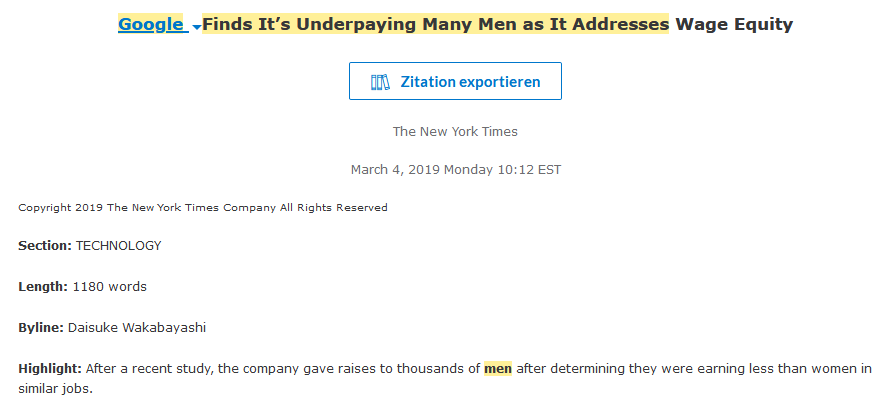
\includegraphics[scale=0.3]{../04-figures/04/04-05}
		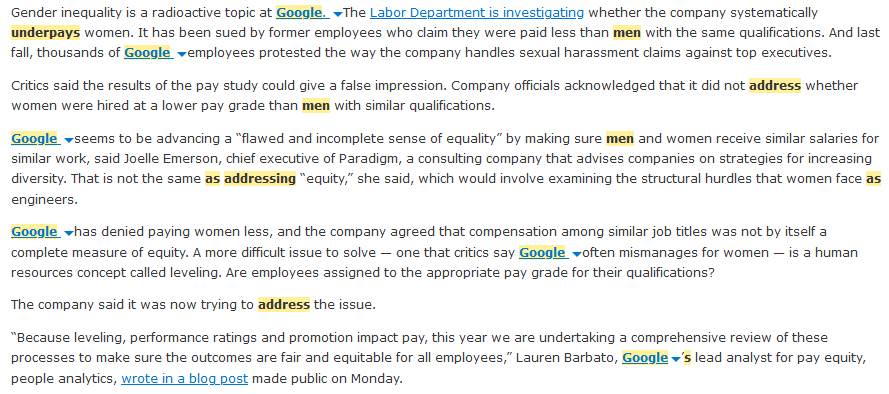
\includegraphics[scale=0.3]{../04-figures/04/04-06}
	\end{figure}
\end{frame}


\section{Conclusion}

\begin{frame}
	\frametitle{Benefits of DAGs}
	DAGs are great to help you make your assumptions clear to your audience.\bigskip
	
	\pause
	
	They also let you understand whether an effect can be causally identified or not, if an assumed model about the world is true.\bigskip
	
	\pause
	
	The NATE is identified if all open back-door paths are closed.
\end{frame}


\begin{frame}
	\frametitle{Benefits of DAGs}
	Conditioning on confounders closes open back-door paths.\bigskip
	
	\pause
	
	DAGs help you choose the right conditioning strategy for your analysis.\bigskip
	
	\pause
	
	Valuable throughout, but especially at early stages of research design:
	
	\begin{itemize}
		\item to understand what needs to be measured
		
		\pause
		
		\item to determine whether effect is causally identified
	\end{itemize}
	
\end{frame}


% END
\begin{frame}
\begin{center}
    \Huge Thank \textcolor{orange}{you} for the kind attention!
\end{center}
\end{frame}

% REFERENCES %

\begin{frame}
\frametitle{References}
\bibliographystyle{apacite}
\bibliography{../Bibliography}
\vspace{5cm}
\end{frame}

\end{document}
